% Options for packages loaded elsewhere
\PassOptionsToPackage{unicode}{hyperref}
\PassOptionsToPackage{hyphens}{url}
%
\documentclass[
  8pt,
  ignorenonframetext,
]{beamer}
\usepackage{pgfpages}
\setbeamertemplate{caption}[numbered]
\setbeamertemplate{caption label separator}{: }
\setbeamercolor{caption name}{fg=normal text.fg}
\beamertemplatenavigationsymbolsempty
% Prevent slide breaks in the middle of a paragraph
\widowpenalties 1 10000
\raggedbottom
\setbeamertemplate{part page}{
  \centering
  \begin{beamercolorbox}[sep=16pt,center]{part title}
    \usebeamerfont{part title}\insertpart\par
  \end{beamercolorbox}
}
\setbeamertemplate{section page}{
  \centering
  \begin{beamercolorbox}[sep=12pt,center]{part title}
    \usebeamerfont{section title}\insertsection\par
  \end{beamercolorbox}
}
\setbeamertemplate{subsection page}{
  \centering
  \begin{beamercolorbox}[sep=8pt,center]{part title}
    \usebeamerfont{subsection title}\insertsubsection\par
  \end{beamercolorbox}
}
\AtBeginPart{
  \frame{\partpage}
}
\AtBeginSection{
  \ifbibliography
  \else
    \frame{\sectionpage}
  \fi
}
\AtBeginSubsection{
  \frame{\subsectionpage}
}
\usepackage{amsmath,amssymb}
\usepackage{lmodern}
\usepackage{iftex}
\ifPDFTeX
  \usepackage[T1]{fontenc}
  \usepackage[utf8]{inputenc}
  \usepackage{textcomp} % provide euro and other symbols
\else % if luatex or xetex
  \usepackage{unicode-math}
  \defaultfontfeatures{Scale=MatchLowercase}
  \defaultfontfeatures[\rmfamily]{Ligatures=TeX,Scale=1}
\fi
% Use upquote if available, for straight quotes in verbatim environments
\IfFileExists{upquote.sty}{\usepackage{upquote}}{}
\IfFileExists{microtype.sty}{% use microtype if available
  \usepackage[]{microtype}
  \UseMicrotypeSet[protrusion]{basicmath} % disable protrusion for tt fonts
}{}
\makeatletter
\@ifundefined{KOMAClassName}{% if non-KOMA class
  \IfFileExists{parskip.sty}{%
    \usepackage{parskip}
  }{% else
    \setlength{\parindent}{0pt}
    \setlength{\parskip}{6pt plus 2pt minus 1pt}}
}{% if KOMA class
  \KOMAoptions{parskip=half}}
\makeatother
\usepackage{xcolor}
\newif\ifbibliography
\setlength{\emergencystretch}{3em} % prevent overfull lines
\providecommand{\tightlist}{%
  \setlength{\itemsep}{0pt}\setlength{\parskip}{0pt}}
\setcounter{secnumdepth}{-\maxdimen} % remove section numbering
% type setting
% ------------------------------------------------------------------------------
\usepackage[german]{babel}     

% fonts
% ------------------------------------------------------------------------------
\usefonttheme{professionalfonts}

% slide title and horizontal line
% ------------------------------------------------------------------------------
\setbeamertemplate{frametitle}{%
    \vskip-30pt \color{black}\large%
    \begin{minipage}[b][23pt]{120mm}%
    \flushleft\insertframetitle%
    \end{minipage}%
}

\setbeamertemplate{headline}										
{
\vskip10pt\hfill\hspace{3.5mm} 										 
\vskip15pt\color{black}\rule{\textwidth}{0.4pt} 					 
}

% slide number
% ---------------------------------------------------------------
\setbeamertemplate{navigation symbols}{}
\setbeamertemplate{footline}
{
\vskip5pt
\vskip2pt
\makebox[123mm]{\hspace{7.5mm}
\hfill Psychologische Forschungsmethoden $\vert$ 
\copyright $ $ 2023 Dirk Ostwald CC BY-SA 4.0 $\vert$ 
Folie \insertframenumber}
\vskip4pt
}

% block color scheme
% ------------------------------------------------------------------------------
% colors
\definecolor{white}{RGB}{255,255,255}
\definecolor{grey}{RGB}{235,235,235}
\definecolor{lightgrey}{RGB}{245,245,245}
\definecolor{LightBlue}{RGB}{220,220,255}
\definecolor{darkblue}{RGB}{51, 51, 153}

% definitions and theorems
\setbeamercolor{block title}{fg = black, bg = grey}
\setbeamercolor{block body}{fg = black, bg = lightgrey}

% general line spacing 
% ------------------------------------------------------------------------------
\linespread{1.3}

% local line spacing
% ------------------------------------------------------------------------------
\usepackage{setspace}

% colors
% -----------------------------------------------------------------------------
\usepackage{color}

% justified text
% ------------------------------------------------------------------------------
\usepackage{ragged2e}
\usepackage{etoolbox}
\apptocmd{\frame}{}{\justifying}{}

% bullet point lists
% -----------------------------------------------------------------------------
\setbeamertemplate{itemize item}[circle]
\setbeamertemplate{itemize subitem}[circle]
\setbeamertemplate{itemize subsubitem}[circle]
\setbeamercolor{itemize item}{fg = black}
\setbeamercolor{itemize subitem}{fg = black}
\setbeamercolor{itemize subsubitem}{fg = black}
\setbeamercolor{enumerate item}{fg = black}
\setbeamercolor{enumerate subitem}{fg = black}
\setbeamercolor{enumerate subsubitem}{fg = black}
\setbeamerfont{itemize/enumerate body}{}
\setbeamerfont{itemize/enumerate subbody}{size = \normalsize}
\setbeamerfont{itemize/enumerate subsubbody}{size = \normalsize}

% color links
% ------------------------------------------------------------------------------
\usepackage{hyperref}
\definecolor{urls}{RGB}{204,0,0}
\hypersetup{colorlinks, citecolor = darkblue, urlcolor = urls}


% additional math commands
% ------------------------------------------------------------------------------
\usepackage{bm}                                         % bold math symbols
\newcommand{\niton}{\not\owns}
\usepackage{cancel} 

% text highlighting
% ------------------------------------------------------------------------------
\usepackage{soul}
\makeatletter
\let\HL\hl
\renewcommand\hl{%
  \let\set@color\beamerorig@set@color
  \let\reset@color\beamerorig@reset@color
  \HL}
\makeatother

% equation highlighting
% -----------------------------------------------------------------------------
\newcommand{\highlight}[2][yellow]{\mathchoice%
  {\colorbox{#1}{$\displaystyle#2$}}%
  {\colorbox{#1}{$\textstyle#2$}}%
  {\colorbox{#1}{$\scriptstyle#2$}}%
  {\colorbox{#1}{$\scriptscriptstyle#2$}}}%

% additional mathematical operators
% ------------------------------------------------------------------------------
\DeclareMathOperator*{\argmax}{arg\,max}
\DeclareMathOperator*{\argmin}{arg\,min}

\ifLuaTeX
  \usepackage{selnolig}  % disable illegal ligatures
\fi
\IfFileExists{bookmark.sty}{\usepackage{bookmark}}{\usepackage{hyperref}}
\IfFileExists{xurl.sty}{\usepackage{xurl}}{} % add URL line breaks if available
\urlstyle{same} % disable monospaced font for URLs
\hypersetup{
  hidelinks,
  pdfcreator={LaTeX via pandoc}}

\author{}
\date{\vspace{-2.5em}}

\begin{document}

\begin{frame}[plain]{}
\protect\hypertarget{section}{}
\center

\begin{center}
\includegraphics[width=0.2\linewidth]{8_Abbildungen/pfm_8_otto} \end{center}

\vspace{2mm}

\Large

Psychologische Forschungsmethoden \vspace{6mm}

\normalsize

BSc Philosophie-Neurowissenschaften-Kognition WiSe 2022/23

BSc Psychologie WiSe 2022/23

\large
\vspace{6mm}

Prof.~Dr.~Dirk Ostwald
\end{frame}

\begin{frame}[plain]{}
\protect\hypertarget{section-1}{}
\vfill
\center
\huge

\textcolor{black}{(8) Ordinalmessung} \vfill
\end{frame}

\begin{frame}{}
\protect\hypertarget{section-2}{}
\Large
\setstretch{3}
\vfill

\textbf{Vorbemerkungen}

Strenge schwache Ordnungen

Repräsentation und Eindeutigkeit

Selbstkontrollfragen \vfill
\end{frame}

\begin{frame}{Vorbemerkungen}
\protect\hypertarget{vorbemerkungen}{}
\textcolor{darkblue}{Vorgehensweisen messtheoretischer Überlegungen}

\small

\(\Rightarrow\) Vom qualitativen Relationssystem zum Homomorphismus und
numerischen Relationssystem

\begin{center}\includegraphics[width=0.7\linewidth]{8_Abbildungen/pfm_8_messtheorie_ansätze} \end{center}

\small

\(\Leftarrow\) Vom numerischen Relationssystem und Homomorphismus zum
qualitativen Relationssystem
\end{frame}

\begin{frame}{Vorbemerkungen}
\protect\hypertarget{vorbemerkungen-1}{}
\textcolor{darkblue}{Vorgehensweisen messtheoretischer Überlegungen}

\small

\(\Rightarrow\) Vom qualitativen Relationssystem zum Homomorphismus und
numerischen Relationssystem

\footnotesize

\justifying Im Anwendungskontext stellt man sich vor, dass ein
bestimmter Gegenstandsbereich als qualitatives Relationssystem mit
bestimmten Eigenschaften beschrieben werden kann. Letztlich sind die
Eigenschaften empirisch zu überprüfen, dafür bietet die klassische
Messtheorie aber keine Methodik. Man legt also ein in gewisser Weise
idealisiertes qualitatives Relationssystem zugrunde und fragt dann, ob
es einen Homomorphismus in ein numerisches Relationssystem, z.B.
\((\mathbb{R},>)\) oder \((\mathbb{R},>,+)\) geben kann. Insgesamt hat
dieser Ansatz sicherlich einen hohen intuitiven Appeal.

\small

\(\Leftarrow\) Vom numerischen Relationssystem und Homomorphismus zum
qualitativen Relationssystem

\footnotesize

Im Theoriekontext fragt man dagegen oft, wenn man ein bestimmtes
numerisches Relationssystem, z.B. \((\mathbb{R},>)\) oder
\((\mathbb{R},>,+)\) und die Existenz eines Homomorphismus zugrundelegt,
welche Eigenschaften dann ein qualitatives Relationssystem mindestens
genügen muss. Dementsprechend geht es einerseits darum, numerische
Relationen wie \(>\) oder \(\ge\) oder Operationen wie \(+\) auf den
reellen Zahlen mithilfe qualitativer Relationsbegriffe zu beschreiben.
Dies motiviert dann z.B. Beispiel die Charakterisierung von
(qualitativen) Ordnungsrelationen. Zum anderen versucht man, nur eben
jene Eigenschaften von qualitativen Relationssystemen zu fordern, die
für den Nachweis der Existenz eines Homomorphismus in ein bestimmtes
numerisches Relationssystem oder die so induzierte Skalenart gerade
nötig sind. Der intuitive Appeal dieser Herangehensweise ist sicherlich
geringer, die erreichbare formale Strenge und Einfachheit jedoch
leichter gewährleistet als im obigem Ansatz. Die Inhalte der Einheiten
zu Ordinalmessungen, Extensivmessungen und Differenzmessungen sollten
auch vor dem Hintergrund dieses zweiten Ansatzes rezipiert werden.
\end{frame}

\begin{frame}{Vorbemerkungen}
\protect\hypertarget{vorbemerkungen-2}{}
\textcolor{darkblue}{Ordnungsrelationen}

\footnotesize

Ziel der Ordinalmessung ist die strukturerhaltende Repräsentation von
\emph{Ordnungsrelationen}. Ordnungsrelationen sind Binärrelationen und
formalisieren Intuitionen von Rangfolgen wie z.B. ``größer als'', ``mehr
als'' oder ``wird präferiert über''. Vertraute Ordnungsrelationen sind
\(>\) und \(\ge\) auf der Menge der reellen Zahlen.

Die \(>\) und \(\ge\) Relationen auf den reellen Zahlen haben
unterschiedliche Eigenschaften. Zum Beispiel ist die Relation \(>\)
nicht reflexiv, weil \(x \cancel{>} x\), also \((x,x) \notin \, >\),
aber die Relation \(\ge\) ist reflexiv, weil \(x \ge x\), also
\((x,x) \in\, \ge\).

Die Theorie der Ordnungsrelationen versucht, Eigenschaften wie die
(Ir)Reflexivität von \(>\) und \(\ge\) zu abstrahieren und auf andere,
nicht numerische Mengen, zu übertragen. Je nach den konkreten
Eigenschaften einer Ordnungsrelation definiert man zum Beispiel folgende
Ordnungsrelationen (aus Roberts (1984), S. 15):

\begin{center}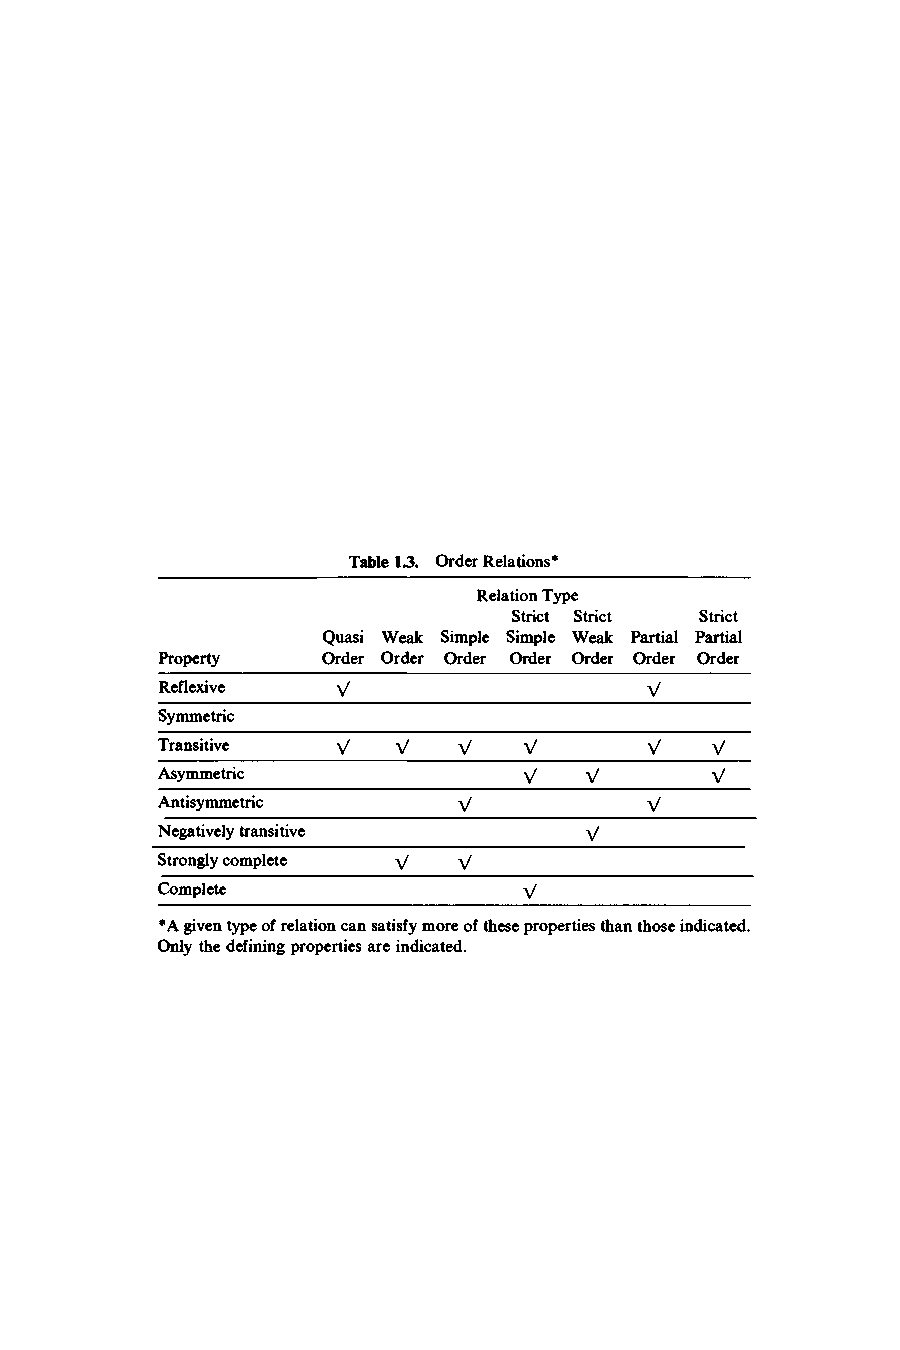
\includegraphics[width=0.4\linewidth]{8_Abbildungen/pfm_8_order_relations} \end{center}

Für jeder der in der Tabelle angegebenen Ordnungsrelationen können das
Repräsentationsproblem und das Eindeutigkeitsproblem der Ordinalmessung
untersucht werden. Wir betrachten hier der Einfachheit halber nur den
Fall der Ordinalmessung bei Vorliegen einer \textbf{strengen schwachen
Ordnung} (strict weak order).
\end{frame}

\begin{frame}{Vorbemerkungen}
\protect\hypertarget{vorbemerkungen-3}{}
\vspace{1mm}

\textcolor{darkblue}{Ordinalmessungen}

\footnotesize

Ziel von Ordinalmessungen ist es, den Elementen einer Menge \(M\), die
in einer gegebenen Ordnungsrelation \(R\) stehen, durch eine Funktion
\(f\) Zahlen in \(\mathbb{R}\) so zuzuordnen, dass gilt \begin{equation}
(m,n) \in R \Leftrightarrow f(m) > f(n)  
\end{equation} oder, in Abhängigkeit von \(R\), auch \begin{equation}
(m,n) \in R \Leftrightarrow f(m) \ge f(n).  
\end{equation} Da die Struktur von \(R\) durch den Homomorphismus per
Definition nicht verändert wird, die Funktion \(f\) also keine
zusätzliche Information im Vergleich zu \(R\) enkodiert, stellt sich die
Frage, was durch eine Ordinalmessung bei bekannter Ordnungsrelation
\(R\) wissenschaftlich überhaupt gewonnen wird.

Mögliche Antworten auf diese Frage sind folgende:

\begin{itemize}
\tightlist
\item
  \justifying \((m,n) \in R \vee (m,n) \notin R\) sind binäre Aussagen,
  \(f(m), f(n) \in \mathbb{R}\) sind Zahlen. Die Übersetzung einer
  qualitativen Ordnungsrelation erlaubt es also, die Methoden der
  angewandten Mathematik auf die numerisch repräsentierte
  Ordnungsrelation anzuwenden. Die den Elementen von \(M\) zugeordneten
  Funktionswerte \(f(m) \in \mathbb{R}\) können zum Beispiel im Sinne
  von abhängigen Variablen mit anderen den Elementen von \(M\)
  zugeordneten Funktionswerten \(g(m) \in \mathbb{R}\) als unabhängige
  Variablen statistisch in Bezug gesetzt werden.
\item
  In ähnlicher Weise sind Antworten auf Fragen der relativen Position
  eines \(m \in M\) unter Umständen anhand der Menge der \(f(m)\)
  leichter zu evaluieren. Zum Beispiel müssen für das ranghöchste oder
  rangniedrigste \(m \in M\) lediglich \(\mbox{argmin}_{m \in M}f(m)\)
  und \(\mbox{argmax}_{m \in M}f(m)\) evaluiert und nicht alle
  paarweisen Vergleiche gezogen werden.
\item
  \((m,n) \in R \vee (m,n) \notin R\) sind \(|M^2|\) Aussagen, \(f(m)\)
  sind \(|M|\) Zahlen. Die numerisch repräsentierte Ordnungsrelation
  kann also eventuell mit weniger Aufwand enkodiert werden.
\end{itemize}
\end{frame}

\begin{frame}{Vorbemerkungen}
\protect\hypertarget{vorbemerkungen-4}{}
\textcolor{darkblue}{Überblick}

\footnotesize

\begin{itemize}
\item
  \justifying Wir geben in dieser Einheit einen Überblick zu
  messtheoretischen Überlegungen zur Repräsentation und Eindeutigkeit
  von strengen schwachen Ordnungen.
\item
  \justifying Im Abschnitt \textbf{Strenge schwache Ordnungen} führen
  wir mit der Asymmetrie und der negativen Transitivität zunächst die
  definierenden Eigenschaften strenger schwacher Ordungen ein. Weiterhin
  zeigen wir, dass strenge schwache Ordnungen auch immer irreflexive und
  transitive Ordnungsrelationen sind.
\item
  Im Abschnitt \textbf{Repräsentation und Eindeutigkeit} zeigen wir
  zunächst, dass für eine strenge schwache Ordnung \(R\) auf einer Menge
  \(M\) immer ein Homomorphismus in das numerische Relationssystem
  \((\mathbb{R}, >)\) existiert und geben damit für den betrachteten
  Fall eine Antwort auf das Repräsentationsproblem der Messtheorie.
  Insbesondere konstruieren wir sogar einen Homomorphismus.
\item
  Im gleichen Abschnitt zeigen wir dann weiterhin, dass der konstruierte
  Homomorphismus nicht eindeutig ist und durch die Klasse der monoton
  steigenden Funktionen in weitere Homomorphismen vom betrachteten
  qualitatitven Relationssystem in das betrachtete numerische
  Relationssysteme transformiert werden kann. Die Klasse der zulässigen
  Transformationen von Homomorphismen sind im vorliegenden Fall also die
  monoton steigenden Funktionen. Damit haben wir dann auch die
  Ordinalskalenart der Repräsentation strenger schwacher Ordnungen
  nachgewiesen.
\item
  Schließlich geben wir ein Anwendungsbeispiel aus dem Bereich der
  Präferenzmessung.
\end{itemize}
\end{frame}

\begin{frame}{}
\protect\hypertarget{section-3}{}
\Large
\setstretch{3}
\vfill

Vorbemerkungen

\textbf{Strenge schwache Ordnungen}

Repräsentation und Eindeutigkeit

Selbstkontrollfragen \vfill
\end{frame}

\begin{frame}{Strenge schwache Ordnungen}
\protect\hypertarget{strenge-schwache-ordnungen}{}
\small
\begin{definition}[Asymmetrie]
Eine Binärrelation $R$ auf einer Menge $M$ heißt \textit{asymmetrisch}, wenn
für alle $(m,n) \in R$ gilt, dass $(n,m) \notin R$ ist.
\end{definition}

\footnotesize

Bemerkungen und Beispiele

\begin{itemize}
\tightlist
\item
  Die \(>\) Relation auf \(\mathbb{R}\) ist asymmetrisch, weil für alle
  \(x,y\in \mathbb{R}\) gilt, dass wenn \(x>y\) gilt, auch
  \(y\cancel{>}x\) gilt.
\item
  Die \(\ge\) Relation auf \(\mathbb{R}\) ist nicht asymmetrisch, weil
  für \(x = y\) bei \(x\ge y\) nicht gilt, dass \(y\cancel{\ge}x\).
\item
  Für \(M := \{a,b,c\}\) ist die Relation \begin{equation}
  R := \{(a,b), (a,c), (b,c)\}
  \end{equation} asymmetrisch, weil gilt, dass \begin{align}
  \begin{split}
  (a,b) \in R & \Rightarrow (b,a) \notin R \\
  (a,c) \in R & \Rightarrow (c,a) \notin R \\
  (b,c) \in R & \Rightarrow (c,b) \notin R \\
  \end{split}
  \end{align}
\item
  Die (rationale, normative, idealisierte) Präferenzrelation ``wird
  präferiert über'' ist asymmetrisch.
\item
  Die Präferenzrelation ``wird präferiert über oder wird gleichermaßen
  präferiert'' ist nicht asymmetrisch.
\end{itemize}
\end{frame}

\begin{frame}{Strenge schwache Ordnungen}
\protect\hypertarget{strenge-schwache-ordnungen-1}{}
\small
\begin{definition}[Negative Transitivität]
\justifying
Eine Binärrelation $R$ auf einer Menge $M$ heißt \textit{negativ transitiv}, wenn
für alle $m,n,p\in M$ gilt, dass aus $(m,n) \notin R$ und $(n,p)\notin R$ folgt,
dass $(m,p) \notin R$ ist.
\end{definition}

\footnotesize

Bemerkungen und Beispiele

\begin{itemize}
\tightlist
\item
  \justifying Die \(>\) Relation auf \(\mathbb{R}\) ist negativ
  transitiv, weil für alle \(x,y,z\in \mathbb{R}\) gilt, dass aus
  \(x\cancel{>}y\) und \(y\cancel{>}z\) folgt, dass \(x\cancel{>}z\).
  Seien zum Beispiel \(x = 1, y = 3\) und \(z = 6\). Offenbar gelten
  dann \(x \cancel{>} y\) und \(y \cancel{>} z\) und auch
  \(x \cancel{>} z\).
\item
  Für \(M := \{a,b,c\}\) ist die Relation \begin{equation}
  R := \{(a,b), (a,c), (b,c)\}
  \end{equation} negativ transitiv. Hier gilt zum Beispiel, dass mit
  \((c,b)\notin R\) und \((b,a) \notin R\) auch \((c,a) \notin R\) ist.
  Für einen vollständigen Nachweis der negativen Transitivität muss
  allerdings gezeigt werden, dass dies für alle relevanten Paare von
  Tupeln in \(M\times M\) gilt.
\item
  Die (rationale, normative, idealisierte) Präferenzrelation ``wird
  präferiert über'' ist negativ transitiv.
\end{itemize}
\end{frame}

\begin{frame}{Strenge schwache Ordnungen}
\protect\hypertarget{strenge-schwache-ordnungen-2}{}
\small
\begin{definition}[Strenge schwache Ordnung]
$M$ sei eine Menge und $R$ sei eine Binärrelation auf $M$. $R$ heißt \textit{strenge schwache Ordnung}
auf $M$, wenn $R$ asymmetrisch und negativ transitiv ist.
\end{definition}
\footnotesize

Bemerkungen und Beispiele

\begin{itemize}
\tightlist
\item
  \justifying Wir haben oben gesehen, dass die \(>\) Relation auf
  \(\mathbb{R}\) asymmetrisch und negativ transitiv ist. Die \(>\)
  Relation ist also eine strenge schwache Ordnung auf \(\mathbb{R}\).
\item
  Wir haben oben auch gesehen, dass die \(\ge\) Relation auf
  \(\mathbb{R}\) nicht asymmetrisch ist. Die \(\ge\) Relation ist also
  keine strenge schwache Ordnung auf \(\mathbb{R}\).
\item
  Wir haben oben angemerkt, dass eine (rationale, normative,
  idealisierte) Präferenzrelation asymmetrisch und negativ transitiv und
  damit eine strenge schwache Ordnung ist.
\end{itemize}
\end{frame}

\begin{frame}{Strenge schwache Ordnungen}
\protect\hypertarget{strenge-schwache-ordnungen-3}{}
\small
\begin{theorem}[Irreflexivität und Transitivität strenger schwacher Ordnung]
\normalfont
Eine strenge schwache Ordnung $R$ auf einer Menge $M$ ist irreflexiv und transitiv.
\end{theorem}

\footnotesize

\underline{Beweis}

Zum Nachweis der Irreflexivität ist zu zeigen, dass für alle \(m \in M\)
gilt, dass \((m,m)\notin R\) ist. Zum Beweis durch Widerspruch sei
\((m,m) \in R\). Dann würde mit der Asymmetrie von \(R\) gelten, dass
mit \((m,m) \in R\) auch \((m,m) \notin R\) ist (um das einzusehen
ersetze man in der Definition der Asymmetrie \(n\) durch \(m\)) und dies
ist ein Widerspruch. Also kann \((m,m) \in R\) nicht gelten und es muss
\((m,m) \notin R\) gelten. Also ist \(R\) irreflexiv.

Zum Nachweis der Transitivität von \(R\) ist zu zeigen, dass für
\((m,n) \in R\) und \((n,p) \in R\) auch \((m,p) \in R\) gilt. Es seien
also \((m,n) \in R\) und \((n,p) \in R\). Zum Beweis durch Widerspruch
sei \((m,p) \notin R\). Die Asymmetrie von \(R\) impliziert, dass aus
\((n,p) \in R\) folgt, dass \((p,n) \notin R\). Die negative
Transitivität von \(R\) impliziert nun für \((m,p) \notin R\) und
\((p,n) \notin R\), dass \((m,n) \notin R\), was ein Widerspruch zur
Voraussetzung \((m,n) \in R\) ist. Also kann \((m,p) \notin R\) nicht
gelten und es muss für \((m,n) \in R\) und \((n,p) \in R\) gelten, dass
\((m,p) \in R\) ist. Also ist \(R\) transitiv.

\(\hfill \Box\)
\end{frame}

\begin{frame}{}
\protect\hypertarget{section-4}{}
\Large
\setstretch{3}
\vfill

Vorbemerkungen

Strenge schwache Ordnungen

\textbf{Repräsentation und Eindeutigkeit}

Selbstkontrollfragen \vfill
\end{frame}

\begin{frame}{Repräsentation und Eindeutigkeit}
\protect\hypertarget{repruxe4sentation-und-eindeutigkeit}{}
\small
\begin{theorem}[Repräsentation strenger schwacher Ordnungen]
\justifying
\normalfont
$\mathcal{M} := (M,R)$ sei ein qualitatives Relationssystem mit einer endlichen Menge
$M$ und einer Binärrelation $R$ auf $M$ und $\mathcal{N} := (\mathbb{R},>)$ sei
ein numerische Relationssystem. Dann existiert ein Homomorphismus $f$ von
$\mathcal{M}$ nach $\mathcal{N}$, also eine Funktion der Form
\begin{equation}
f : M \to \mathbb{R}, m \mapsto f(m)
\end{equation}
mit der Eigenschaft
\begin{equation}
(m,n) \in R \Leftrightarrow f(m) > f(n)
\end{equation}
dann und nur dann, wenn $R$ eine strenge schwache Ordnung ist.
\end{theorem}

\footnotesize

Bemerkungen

\begin{itemize}
\tightlist
\item
  Das Theorem beantwortet das Repräsentationsproblem für die hier
  betrachteten Fälle von \(\mathcal{M}\) und \(\mathcal{N}\).
\item
  Für eine strenge schwachen Ordnung auf einer endlichen Menge sind
  \((M,R)\) und \((\mathbb{R},>)\) also homomorph.
\end{itemize}
\end{frame}

\begin{frame}{Repräsentation und Eindeutigkeit}
\protect\hypertarget{repruxe4sentation-und-eindeutigkeit-1}{}
\footnotesize

\underline{Beweis}

Wir zeigen in einem ersten Schritt, dass wenn ein Homomorphismus von
\((M,R)\) nach \((\mathbb{R},>)\) existiert, \(R\) eine strenge schwache
Ordnung sein muss. In einem zweiten Schritt zeigen wir dann, dass wenn
\(R\) eine strenge schwache Ordnung ist, ein Homomorphismus von
\((M,R)\) nach \((\mathbb{R}, >)\) konstruiert werden kann.

\noindent (1) \emph{Ein Homomorphismus \(f\) von \((M,R)\) nach
\((\mathbb{R},>)\) existiert \(\Rightarrow\) \(R\) muss eine strenge
schwache Ordnung sein}

Wir zeigen, dass aus der Existenz eines Homomorphismus \(f\) von
\((M,R)\) nach \((\mathbb{R},>)\) die Asymmetrie und die negative
Transitivität von \(R\) folgen.

Zum Nachweis der Asymmetrie sei \((m,n) \in R\). Dann gilt nach
Voraussetzung, dass \(f(m) > f(n)\). Da die \(>\) Relation auf
\(\mathbb{R}\) asymmetrisch ist, gilt dann \(f(n) \cancel{>} f(m)\) und
dementsprechend auch \((n,m) \notin R\). Also folgt für alle
\((m,n) \in R\), dass \((n,m) \notin R\) ist und damit ist \(R\)
asymmetrisch.

Zum Nachweis der negativen Transitivität seien \((m,n)\notin R\) und
\((n,p)\notin R\). Dann gelten \(f(m)\cancel{>}f(n)\) und
\(f(n)\cancel{>}f(p)\). Dann folgt aber auch \(f(m)\cancel{>}f(p)\) und
dementsprechend auch \((n,p) \notin R\).

Die Existenz eines Homomorphismus von \((M,R)\) nach \((\mathbb{R},>)\)
impliziert also, dass \(R\) eine strenge schwache Ordnung auf \(M\) ist.
\end{frame}

\begin{frame}{Repräsentation und Eindeutigkeit}
\protect\hypertarget{repruxe4sentation-und-eindeutigkeit-2}{}
\footnotesize

\underline{Beweis (fortgeführt)}

\noindent (2) \emph{\(R\) ist eine strenge schwache Ordnung auf \(M\)
\(\Rightarrow\) Ein Homomorphismus \(f\) kann konstruiert werden}

Wir zeigen, dass für ein qualitatives Relationssystem \((M,R)\) aus
einer endlichen Menge \(M\) und einer strengen schwachen Ordnung \(R\)
ein Homomorphismus von \((M,R)\) nach \((\mathbb{R},>)\) konstruiert
werden kann. Wir definieren dazu eine Funktion \(f\) wie folgt:
\begin{equation}
f : M \to \mathbb{R}, m \mapsto f(m) := |\{q \in M|(m,q) \in R\}| 
\end{equation} Der einem Element \(m \in M\) zugeordnete Funktionswert
\(f(m)\) soll also die Kardinalität der Menge der \(q \in M\) sein, für
die gilt, dass \((m,q) \in R\).

Zum Beispiel sei für \(M := \{a,b,c,d\}\) die strenge schwache Ordnung
\begin{equation}
R := \{(a,c), (a,d), (b,c), (b,d), (c,d)\}
\end{equation} definiert. Dann gilt für \(f\), dass \begin{align}
\begin{split}
f(a) = 2 & \mbox{, weil } \{q \in M|(a,q) \in R\} = \{c,d\}    \\
f(b) = 2 & \mbox{, weil } \{q \in M|(b,q) \in R\} = \{c,d\}    \\
f(c) = 1 & \mbox{, weil } \{q \in M|(c,q) \in R\} = \{d\}      \\
f(d) = 0 & \mbox{, weil } \{q \in M|(d,q) \in R\} = \emptyset  \\
\end{split}
\end{align}
\end{frame}

\begin{frame}{Repräsentation und Eindeutigkeit}
\protect\hypertarget{repruxe4sentation-und-eindeutigkeit-3}{}
\footnotesize

\underline{Beweis (fortgeführt)}

Wir zeigen nun, dass ein solch definiertes \(f\) die Forderung
\((m,n) \in R \Leftrightarrow f(m)>f(n)\) erfüllt. Dazu zeigen wir
erstens, dass aus \((m,n) \in R\) folgt, dass \(f(m)>f(n)\) ist und
zweitens, dass (2) as \(f(m)>f(n)\) folgt, dass \((m,n) \in R\) ist.

\noindent (1) \((m,n) \in R \Rightarrow f(m)>f(n)\)

Es sei \((m,n) \in R\). Weil \(R\) transitiv ist, impliziert
\((n,q) \in R\) dann \((m,q) \in R\) für jedes \(q \in M\). Die Anzahl
der \(q\) mit \((m,q) \in R\) ist also mindestens so groß wie die Anzahl
der \(q\) mit \((n,q) \in M\). Es gilt also \begin{equation}
|\{q \in M|(m,q) \in R\}| \ge |\{q \in M|(n,q) \in R\}| \Leftrightarrow f(m) \ge f(n)
\end{equation} Weiterhin gilt aber auch \begin{equation}
|\{q \in M|(m,q) \in R\}| \neq |\{q \in M|(n,q) \in R\}| \Leftrightarrow f(m) \neq f(n),
\end{equation} weil nach Voraussetzung \((m,n) \in R\), aber aufgrund
der Irreflexitivität von \(R\) dann \((n,n) \notin R\) gilt. Für \(n\)
gilt also \begin{equation}
n \in \{q \in M|(m,q) \in R\}, \mbox{ aber } n \notin \{q \in M|(n,q) \in R\}.
\end{equation} Damit können die Kardinalitäten dieser beiden Mengen
nicht gleich sein. Also gilt \((m,n) \in R \Rightarrow f(m)>f(n)\).
\end{frame}

\begin{frame}{Repräsentation und Eindeutigkeit}
\protect\hypertarget{repruxe4sentation-und-eindeutigkeit-4}{}
\footnotesize

\underline{Beweis (fortgeführt)}

\noindent (2) \(f(m)>f(n) \Rightarrow (m,n) \in R\)

Im Folgenden nutzen wir Kontrapositionsbeweise, also die logische
Äquivalenz von \(A \Rightarrow B\) und \(\neg B \Rightarrow \neg A\),
z.B. \begin{equation*}
\mbox{Es regnet } (A)  \Rightarrow \mbox{ Die Strasse ist nass } (B) \Leftrightarrow \mbox{ Die Strasse ist nicht nass } (\neg B)  \Rightarrow  \mbox{ Es regnet nicht } (\neg A).
\end{equation*} Um zu zeigen, dass aus \(f(m)>f(n)\) folgt, dass
\((m,n) \in R\) ist, zeigen wir also, dass umgekehrt aus
\((m,n) \notin R\) folgt, dass \(f(m) \cancel{>} f(n)\). Dazu halten wir
fest, dass aus der negativen Transitivität von \(R\) folgt, dass für
\((m,n) \notin R\) aus \((n,q) \notin R\) folgt, dass
\((m,q) \notin R\). Andersherum impliziert dann aber \((m,q) \in R\),
dass \((n,q) \in R\) ist und damit \begin{equation*}
(m,n) \notin R \Rightarrow |\{q \in M|(n,q) \in R\}| \ge |\{q \in M|(m,q) \in R\}| \Leftrightarrow f(n) \ge f(m) \Leftrightarrow f(m) \cancel{>} f(n).
\end{equation*} Damit ist bewiesen, dass aus \((m,n) \notin R\) folgt,
dass \(f(m) \cancel{>} f(n)\) und äquivalent, dass aus \(f(m)>f(n)\)
folgt, dass \((m,n) \in R\) ist.
\end{frame}

\begin{frame}{Repräsentation und Eindeutigkeit}
\protect\hypertarget{repruxe4sentation-und-eindeutigkeit-5}{}
\small
\begin{theorem}[Eindeutigkeit der Repräsentation strenger schwacher Ordnungen]
\justifying
\normalfont
$\mathcal{M} := (M,R)$ sei ein qualitatives Relationssystem aus einer endlichen Menge
$M$ und einer strengen schwachen Ordnung $R$ auf $M$, $\mathcal{N} := (\mathbb{R},>)$ sei
ein numerische Relationssystem und es sei $f \in \mathcal{H}(\mathcal{M},\mathcal{N})$.
Dann ist $(\mathcal{M},\mathcal{N},f)$ eine Ordinalskala.
\end{theorem}

\footnotesize

Bemerkungen

\begin{itemize}
\tightlist
\item
  Die Klasse der zulässigen Transformationen von \(f\) sind also die
  monoton steigenden Funktionen.
\item
  Dass in diesem Fall
  \(\mathcal{H}(\mathcal{M},\mathcal{N}) \neq \emptyset\) gilt, wurde
  oben nachgewiesen.
\item
  Strenge schwache Ordnungen sind also nicht eindeutig repräsentiert.
\end{itemize}
\end{frame}

\begin{frame}{Repräsentation und Eindeutigkeit}
\protect\hypertarget{repruxe4sentation-und-eindeutigkeit-6}{}
\footnotesize

\underline{Beweis}

\noindent (1) \emph{Regularität der Repräsentation}

Wir zeigen zunächst, dass die Repräsentation
\(\mathcal{M} \to \mathcal{N}\) regulär ist, um nachzuweisen, dass es zu
jedem \(f \in \mathcal{H}(\mathcal{M}, \mathcal{N})\) eine zulässige
Transformation gibt. Dazu nutzen wir das Theorem zur Charakterisierung
regulärer Skalen (vgl. (7) Skalenarten), welches besagt, dass eine Skala
\((\mathcal{M},\mathcal{N},f)\) dann und nur dann regulär ist, wenn für
alle \(g \in \mathcal{H}(\mathcal{M}, \mathcal{N})\) und \(m,n \in M\)
gilt, dass aus \(f(m) = f(n)\) folgt, dass \(g(m) = g(n)\) ist. Sei
also\\
\(g \in \mathcal{H}(\mathcal{M}, \mathcal{N})\), d.h. \(g\) erfüllt die
Eigenschaft \begin{equation}
g : M \to \mathbb{R}, m \mapsto g(m) \mbox{ mit } (m,n) \in R \Leftrightarrow g(m) > g(n).
\end{equation} Sei nun weiterhin \(f(m) = f(n)\). Dies impliziert, dass
\((m,n) \not R\) und \((n,m) \notin R\), weil sonst entweder
\(f(m) > f(n)\) oder \(f(n) > f(m)\) gelten. Wenn aber
\((n,m) \notin R\) und \((m,n) \notin R\), dann können auch weder
\(g(m) > g(n)\) noch \(g(n) > g(m)\) gelten. Also muss \(g(m) = g(n)\)
gelten.

Weil \(f \in \mathcal{H}(\mathcal{M}, \mathcal{N})\) beliebig war, gilt
dies für alle \(f \in \mathcal{H}(\mathcal{M}, \mathcal{N})\) und damit
ist die Repräsentation \(\mathcal{M} \to \mathcal{N}\) regulär und es
gibt zu jedem \(g \in \mathcal{H}(\mathcal{M}, \mathcal{N})\) eine
zulässige Transformation \(\phi\), so dass \(g = \phi \circ f\).
\end{frame}

\begin{frame}{Repräsentation und Eindeutigkeit}
\protect\hypertarget{repruxe4sentation-und-eindeutigkeit-7}{}
\footnotesize
\vspace{1mm}

\underline{Beweis (fortgeführt)}

\noindent (2) \emph{Ordinalskalenart}

Wir zeigen nun, dass die Menge der zulässigen Transformationen von
\((\mathcal{M},\mathcal{N},f)\) die Menge der monoton steigenden
Funktionen ist. Dazu zeigen wir zunächst, dass für eine monoton
steigende Funktion \(\phi\) gilt, dass
\(\phi \circ f \in \mathcal{H}(\mathcal{M}, \mathcal{N})\). Abschließen
zeigen wir, dass aus
\(\phi \circ f \in \mathcal{H}(\mathcal{M}, \mathcal{N})\) folgt, dass
\(\phi\) eine monoton steigende Funktion ist. Dazu halten wir zunächst
noch ein einmal fest, dass für die Verkettung \(\varphi \circ \psi\)
zweier monoton steigender Funktionen \(\varphi\) und \(\psi\) gilt, dass
ihre Verkettung wiederum monoton steigend ist, denn \begin{equation}
x > y \Leftrightarrow \psi(x) > \psi(y) \Leftrightarrow \varphi(\psi(x)) > \varphi(\psi(y))  \Leftrightarrow (\varphi \circ \psi) (x) > (\varphi \circ \psi) (y).
\end{equation}

(2.1) \emph{\(\phi\) ist monoton steigend \(\Rightarrow\)
\(\phi \circ f \in \mathcal{H}(\mathcal{M}, \mathcal{N})\)} Es gilt
\begin{equation}
(m,n) \in R \Leftrightarrow f(m) > f(n) \Leftrightarrow \phi(f(m)) > \phi(f(n)) \Leftrightarrow  (\phi \circ f)(m) >  (\phi \circ f)(n).
\end{equation} Also ist
\(\phi \circ f \in \mathcal{H}(\mathcal{M}, \mathcal{N})\).

(2.2)
\emph{\(\phi \circ f \in \mathcal{H}(\mathcal{M}, \mathcal{N}) \Rightarrow \phi\)
ist monoton steigend}

Es seien \(\mu := f(m) \in f(M)\) und \(\nu := f(n) \in f(M)\). Dann
gilt für \(\phi \circ f \in \mathcal{H}(\mathcal{M}, \mathcal{N})\),
dass \begin{equation}
\mu > \nu \Leftrightarrow f(m) > f(n) \Leftrightarrow m > n  \Leftrightarrow (\phi \circ f)(m) > (\phi \circ f)(n) \Leftrightarrow \phi(\mu) > \phi(\nu).
\end{equation} Also ist \(\phi\) monoton steigend.
\end{frame}

\begin{frame}{Repräsentation und Eindeutigkeit}
\protect\hypertarget{repruxe4sentation-und-eindeutigkeit-8}{}
\textcolor{darkblue}{Anwendungsbeispiel} \footnotesize

Es sei
\(M := \{\mbox{ROP},\mbox{HOTD},\mbox{ST4}, \mbox{OWK}, \mbox{1899}\}\)
eine Menge von Serien und es sei \(R\) die durch untenstehendes Schema
definierte ``wird präferiert über'' strenge schwache Ordnung auf \(M\)
eines Individuums. Dabei enkodiert eine 1 in der \(m,q\)-ten Zelle, dass
\(m\) über \(q\) präferiert wird, also \((m,q) \in R\), eine 0 in der
\(m,q\)-ten Zelle, dass dies nicht gilt, also \((m,q) \notin R\). Die
letzte Spalte zeigt die Funktionswerte des im Beweis der Repräsentation
strenger schwacher Ordnungen konstruierten Homomorphismus.

\vspace{1mm}
\tiny
\center
\begin{tabular}{l|ccccc|c}
$m \downarrow, q \rightarrow$ & ROP   & HOTD  & ST4   & OWK & 1899  & $|\{q \in M| (m,q) \in R \}|$ \\\hline
ROP                           & 0     & 0     & 0     & 1   & 1     & 2                             \\
HOTD                          & 1     & 0     & 1     & 1   & 1     & 4                             \\
ST4                           & 1     & 0     & 0     & 1   & 1     & 3                             \\
OWK                           & 0     & 0     & 0     & 0   & 0     & 0                             \\
1899                          & 0     & 0     & 0     & 1   & 0     & 1                             \\\hline
\end{tabular}

\footnotesize
\flushleft
\vspace{1mm}

Eine Neuanordnung von Zeilen und Spalten anhand obiger Zeilensummen
lässt die Ordnung klarer erkennen: \vspace{1mm}

\tiny
\center
\begin{tabular}{l|ccccc|c}
$m \downarrow, q \rightarrow$ & HOTD  & ST4   & ROP & 1899 & OWK  & $|\{q \in M| (m,q) \in R \}|$ \\\hline
HOTD                          & 0     & 1     & 1   & 1    & 1    & 4                             \\
ST4                           & 0     & 0     & 1   & 1    & 1    & 3                             \\
ROP                           & 0     & 0     & 0   & 1    & 1    & 2                             \\
1899                          & 0     & 0     & 0   & 0    & 1    & 1                             \\
OWK                           & 0     & 0     & 0   & 0    & 0    & 0                             \\\hline
\end{tabular}

\flushleft
\footnotesize
\vspace{1mm}

Für dieses Individuum gilt für alle \(m,n\in M\), dass \(m\) über \(n\)
präferiert wird oder dass \(n\) über \(m\) präferiert wird.
\end{frame}

\begin{frame}{Repräsentation und Eindeutigkeit}
\protect\hypertarget{repruxe4sentation-und-eindeutigkeit-9}{}
\vspace{3mm}

\textcolor{darkblue}{Anwendungsbeispiel} \footnotesize

Elemente von \(\mathcal{H}(\mathcal{M},\mathcal{N})\) im vorliegenden
Beispiel

\begin{center}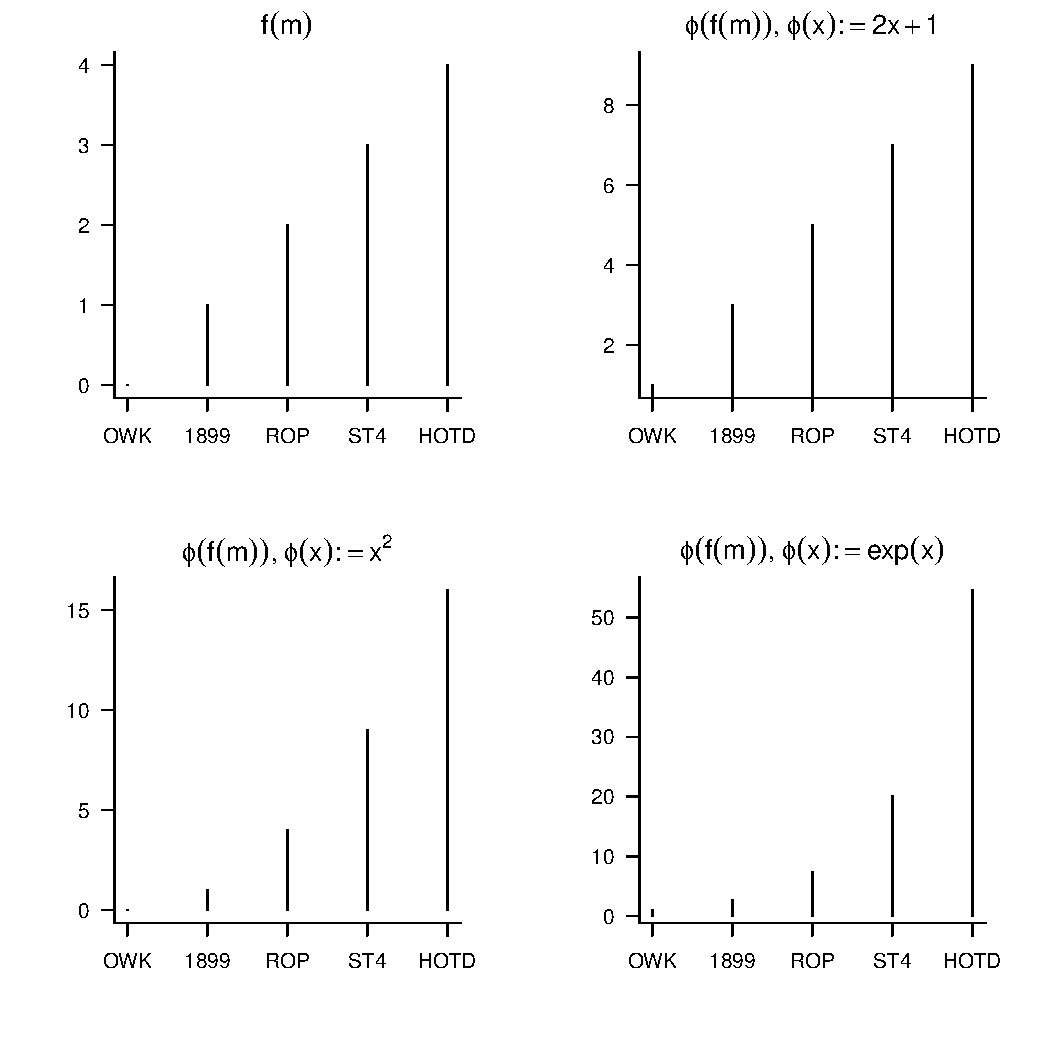
\includegraphics[width=0.62\linewidth]{8_Abbildungen/pfm_8_anwendungsbeispiel} \end{center}
\end{frame}

\begin{frame}{}
\protect\hypertarget{section-5}{}
\Large
\setstretch{3}
\vfill

Vorbemerkungen

Strenge schwache Ordnungen

Repräsentation und Eindeutigkeit

\textbf{Selbstkontrollfragen} \vfill
\end{frame}

\begin{frame}{Selbstkontrollfragen}
\protect\hypertarget{selbstkontrollfragen}{}
\footnotesize
\setstretch{2.2}

\begin{enumerate}
\tightlist
\item
  Erläutern Sie zwei prinzipielle Vorgehensweisen bei messtheoretischen
  Überlegungen.
\item
  Erläutern Sie den Begriff der Ordungsrelation.
\item
  Erläutern Sie das Ziel und den wissenschaftlichen Gewinn von
  Ordinalmessungen.
\item
  Definieren Sie den Begriff der asymmetrischen Binärrelation.
\item
  Definieren Sie den Begriff der negativ transitiven Binärrelation.
\item
  Definieren Sie den Begriff der strengen schwachen Ordnung.
\item
  Geben Sie das Theorem zur Irreflexivität und Transitivität strenger
  schwacher Ordnungen wieder.
\item
  Geben Sie das Theorem zur Repräsentation strenger schwacher Ordnungen
  wieder.
\item
  Geben Sie das Theorem zur Eindeutigkeit strenger schwacher Ordnungen
  wieder.
\item
  Erläutern Sie die Konstruktion eines Homomorphismus von einer strengen
  schwachen Ordnung nach \((\mathbb{R},>)\) anhand eines Beispiels aus
  dem Bereich der Präferenzmessung.
\end{enumerate}
\end{frame}

\end{document}
